\documentclass[nohyper,justified]{tufte-handout}\usepackage[]{graphicx}\usepackage[]{color}
%% maxwidth is the original width if it is less than linewidth
%% otherwise use linewidth (to make sure the graphics do not exceed the margin)
\makeatletter
\def\maxwidth{ %
  \ifdim\Gin@nat@width>\linewidth
    \linewidth
  \else
    \Gin@nat@width
  \fi
}
\makeatother

\definecolor{fgcolor}{rgb}{0.345, 0.345, 0.345}
\newcommand{\hlnum}[1]{\textcolor[rgb]{0.686,0.059,0.569}{#1}}%
\newcommand{\hlstr}[1]{\textcolor[rgb]{0.192,0.494,0.8}{#1}}%
\newcommand{\hlcom}[1]{\textcolor[rgb]{0.678,0.584,0.686}{\textit{#1}}}%
\newcommand{\hlopt}[1]{\textcolor[rgb]{0,0,0}{#1}}%
\newcommand{\hlstd}[1]{\textcolor[rgb]{0.345,0.345,0.345}{#1}}%
\newcommand{\hlkwa}[1]{\textcolor[rgb]{0.161,0.373,0.58}{\textbf{#1}}}%
\newcommand{\hlkwb}[1]{\textcolor[rgb]{0.69,0.353,0.396}{#1}}%
\newcommand{\hlkwc}[1]{\textcolor[rgb]{0.333,0.667,0.333}{#1}}%
\newcommand{\hlkwd}[1]{\textcolor[rgb]{0.737,0.353,0.396}{\textbf{#1}}}%

\usepackage{framed}
\makeatletter
\newenvironment{kframe}{%
 \def\at@end@of@kframe{}%
 \ifinner\ifhmode%
  \def\at@end@of@kframe{\end{minipage}}%
  \begin{minipage}{\columnwidth}%
 \fi\fi%
 \def\FrameCommand##1{\hskip\@totalleftmargin \hskip-\fboxsep
 \colorbox{shadecolor}{##1}\hskip-\fboxsep
     % There is no \\@totalrightmargin, so:
     \hskip-\linewidth \hskip-\@totalleftmargin \hskip\columnwidth}%
 \MakeFramed {\advance\hsize-\width
   \@totalleftmargin\z@ \linewidth\hsize
   \@setminipage}}%
 {\par\unskip\endMakeFramed%
 \at@end@of@kframe}
\makeatother

\definecolor{shadecolor}{rgb}{.97, .97, .97}
\definecolor{messagecolor}{rgb}{0, 0, 0}
\definecolor{warningcolor}{rgb}{1, 0, 1}
\definecolor{errorcolor}{rgb}{1, 0, 0}
\newenvironment{knitrout}{}{} % an empty environment to be redefined in TeX

\usepackage{alltt}
\usepackage[T1]{fontenc}
\usepackage{url}
\usepackage[unicode=true,pdfusetitle,
 bookmarks=true,bookmarksnumbered=true,bookmarksopen=true,bookmarksopenlevel=2,
 breaklinks=true,pdfborder={0 0 1},backref=false,colorlinks=false]
 {hyperref}
\hypersetup{
 pdfstartview=FitH}

\makeatletter

%%%%%%%%%%%%%%%%%%%%%%%%%%%%%% LyX specific LaTeX commands.

\title{MA 2300 Section 2}
\author{Kate Davis}

%%%%%%%%%%%%%%%%%%%%%%%%%%%%%% User specified LaTeX commands.
\renewcommand{\textfraction}{0.05}
\renewcommand{\topfraction}{0.8}
\renewcommand{\bottomfraction}{0.8}
\renewcommand{\floatpagefraction}{0.75}

\usepackage[buttonsize=1em]{animate}

\makeatother
\IfFileExists{upquote.sty}{\usepackage{upquote}}{}
\begin{document}




\maketitle
\section{Introduction to Data Analysis}
Statistical Data Analysis is quantitative evaluation of \textbf{Numeric Data}\marginnote{\textbf{Numeric Data} points are numbers that represents value. Generally, each numeric data point  has a unit of measure} and multiple data points with the same unit can be combined using basic arithmetic operations to form a new data point. Height (in mm), weight (in kg), temperature (degrees F), proportions (percent), and monetary values are examples of  \textbf{continuous}\marginnote{\textbf{Continuous Data} has an infinite number of possible values within a given range, usually represented by real numbers, percentages or fractions} numeric data points. \textbf{Discrete}\marginnote{\textbf{Discrete Data} are data with a finite list of possible values within any given range, and are often integer or count data} numeric data are whole number data or count data, such as the number of sunspots per month, the number of apples in a bushel, or dice roll values.  House numbers, credit scores, and jersey numbers are examples of numbers that are not numeric data points, as none have units nor can these numbers be combined arithmetically to form another numeric data point.

\section{Height in Whole Inches}
Consider the numeric \textbf{Data Set}\marginnote{A \textbf{Data Set} is a collection of numeric data points} of \textbf{Height in Whole Inches} of our \textbf{Population}\marginnote{A \textbf{Population} is any complete group or set of measure with at least one characteristic in common}: students in MA3200 Section 2. Heights would be continuous data, but we have ``discretized'' this data by rounding to the nearest whole inch. The data, in the original order presented, is:

\begin{knitrout}
\definecolor{shadecolor}{rgb}{0.969, 0.969, 0.969}\color{fgcolor}\begin{kframe}
\begin{verbatim}
64 70 72 73 69 67 68 66 62 71 66 72 67 74 71 72 67 71 65 65 69 71 69 72 71 68 63 54
\end{verbatim}
\end{kframe}
\end{knitrout}
This set of data has 28 data points. To better evaluate this data, lets sort it. We\marginnote{The \textbf{Range} is difference between the maximum and minimum values of a data set} can begin to see patterns of multiple values, and can quickly see that the lowest or minimum value is 54 inches and the highest or maximum value is 74 inches. The \textbf{Range} is 20 inches.

\begin{knitrout}
\definecolor{shadecolor}{rgb}{0.969, 0.969, 0.969}\color{fgcolor}\begin{kframe}
\begin{verbatim}
54 62 63 64 65 65 66 66 67 67 67 68 68 69 69 69 70 71 71 71 71 71 72 72 72 72 73 74
\end{verbatim}
\end{kframe}
\end{knitrout}

This data set has 14 discrete values for height, fewer than the range of $20$ inches. There is a gap in observations between $54$ inches and $62$ inches, but all other height values in the range are represented.

To gain more knowledge about this dataset, we must describe the \textbf{distribution}\marginnote{The Oxford English Dictionary defines \textbf{Distribution} as the \textit{way in which something is shared out among a group or spread over an area} } of values across the measurement range, with a goal of using that information for predictions, estimations and other inferences about the population when a complete \textbf{census}\marginnote{A \textbf{Census} is a complete enumeration of every unit, everyone or everything in a population.} 

The \textbf{statistical distribution}\marginnote{A \textbf{Statistical Distribution} assigns probabilities to the possible values of a data set } can be estimated or inferred from a data set, and 
is used to estimate the accuracy of these predictions, estimates, inferences.

\section{Frequency Tables}
We can create a \textbf{Frequency table}\marginnote{a \textbf{Frequency Table} is a summary of data point Frequency by class or interval} and \textbf{histogram}\marginnote{a \textbf{Histogram} is a chart that displays the distribution of a data set} of the data set values. The height data is in whole inches, so we will start with using the integer height value as the class in integer order. A cumulative frequency column is added for additional calculation.

% latex table generated in R 3.1.2 by xtable 1.7-4 package
% Wed Jan 28 21:04:09 2015
\begin{table}[ht]
\centering
\scalebox{0.95}{
\begin{tabular}{rrr}
  \hline
Height & Frequency & CumulativeFrequency \\ 
  \hline
 54 &   1 &   1 \\ 
   62 &   1 &   2 \\ 
   63 &   1 &   3 \\ 
   64 &   1 &   4 \\ 
   65 &   2 &   6 \\ 
   66 &   2 &   8 \\ 
   67 &   3 &  11 \\ 
   68 &   2 &  13 \\ 
   69 &   3 &  16 \\ 
   70 &   1 &  17 \\ 
   71 &   5 &  22 \\ 
   72 &   4 &  26 \\ 
   73 &   1 &  27 \\ 
   74 &   1 &  28 \\ 
   \hline
\end{tabular}
}
\caption{Frequency Table} 
\end{table}


\section{Measures of Center}


To understand more about the distribution of the height in inches of our studens, we first examine ``centers'' of the data: the mode, the median, and the mean.

The \textbf{mode}\marginnote{The \textbf{Mode} of a data set is value that has the highest frequency} of this dataset is 71 inches with frequency 5 students. The mode is easily found from the frequency table. If there is one clear mode in a distribution, the dataset is said to be \textit{unimodal}. A data set can have more than one mode, or be \textit{multi-modal}.

The \textbf{median}\marginnote{The \textbf{median} of a data set is the midpoint of the distribution, or the middle value of the data when sorted in ascending order} of this dataset is 66 inches with frequency of 3 students. If the number $n$ of data points is odd, this is a simple observation of $(n+1)/2$. If the number of data points is even, the arithmetic average of the nearest two data point values is the median.

The \textbf{mean}\marginnote{The \textbf{Mean} of a data set refers to the arithmetic mean of the values} height is 68.17857 inches. The mean is the center that we will use to further examine the ``spread'' of the values.

\begin{knitrout}
\definecolor{shadecolor}{rgb}{0.969, 0.969, 0.969}\color{fgcolor}\begin{figure}

{\centering 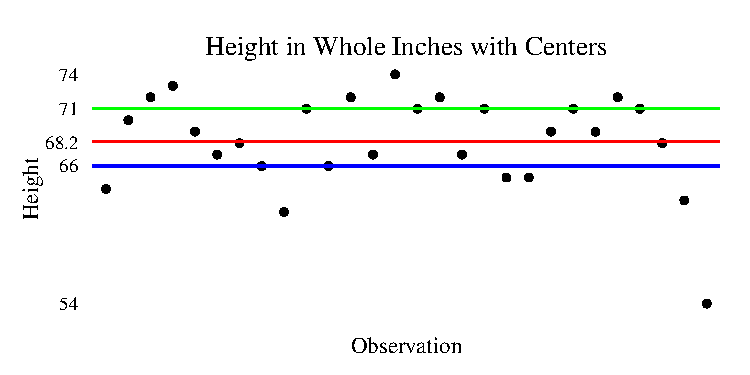
\includegraphics[width=\maxwidth]{figure/graphics-center-chart-1} 

}

\caption[Heights in Observation order with Mode (Green), Median (Blue) and Mean (Red) lines]{Heights in Observation order with Mode (Green), Median (Blue) and Mean (Red) lines}\label{fig:center-chart}
\end{figure}


\end{knitrout}



\section{Distribution Shapes: Histograms, Frequency Polygons, and Ogives}

Once we have calculated the frequencies and centers of our datasets we can start to explore the shape and spread of the distribution of values. 

The \textbf{histogram}\marginnote{A \textbf{Histogram} is a visualization of a frequency table.} is a view of the overall pattern of the distribution. Histogram bars are evenly sized and each bar represents the same class levels of values, and is centered on the mean of the class. The height of the bar represents the number of observations in that class.

The mode can easily be seen on a histogram, and the median is the vertical line at which there is equal area to the left and to the right in the chart. 

A histogram's shape can be symmetric, skewed right with more of the observations on the right or higher values, or skewed to the left with more of the observations on the left or lower values.

A frequency polygon simply displays the frequency for a class, and an ogive, or cumulative frequency polygon displays the cumulative frequency for a class. 

\begin{knitrout}
\definecolor{shadecolor}{rgb}{0.969, 0.969, 0.969}\color{fgcolor}\begin{figure}

{\centering 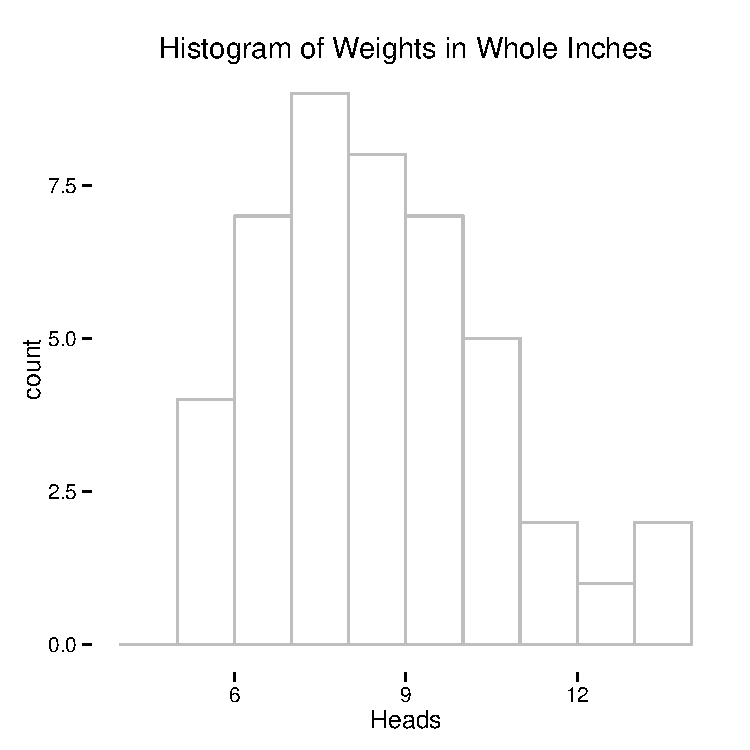
\includegraphics[width=.49\linewidth]{figure/graphics-histogram-1} 
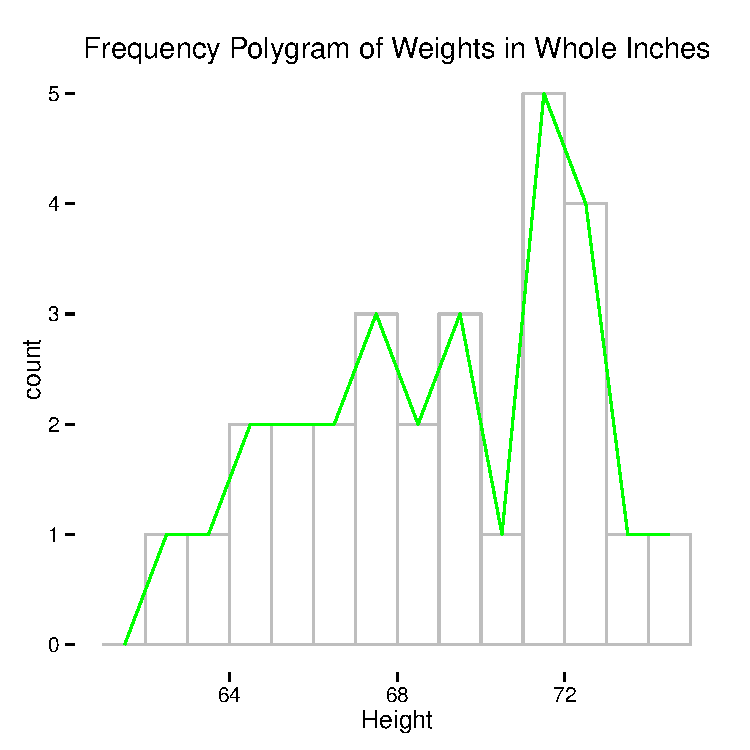
\includegraphics[width=.49\linewidth]{figure/graphics-histogram-2} 

}

\caption[Histograms with Frequency Polygon and Ogive (Cumulative Frequency Polygon)]{Histograms with Frequency Polygon and Ogive (Cumulative Frequency Polygon). The Height data set is unimodal, skewed right, with out outlier on the left. }\label{fig:histogram}
\end{figure}


\end{knitrout}

\begin{knitrout}
\definecolor{shadecolor}{rgb}{0.969, 0.969, 0.969}\color{fgcolor}\begin{figure}

{\centering 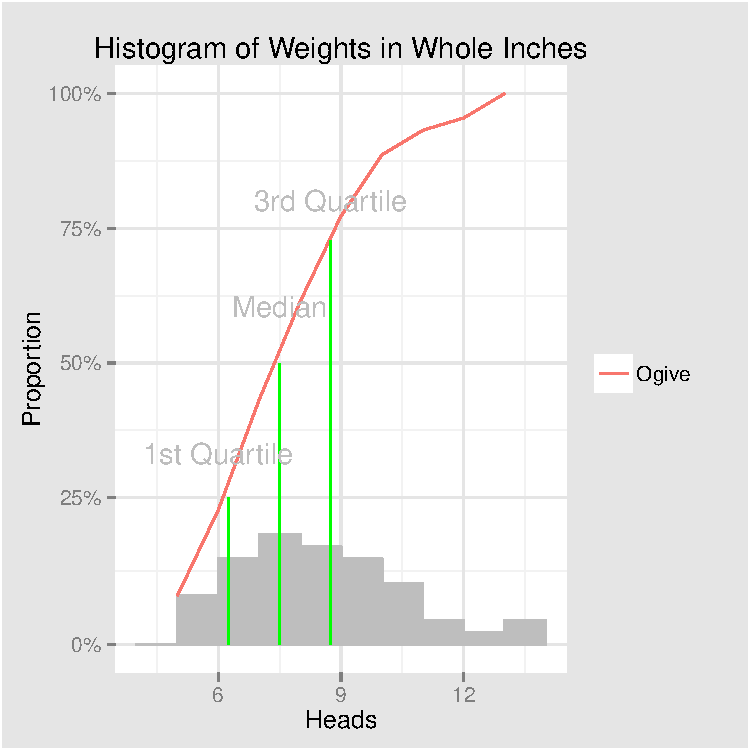
\includegraphics[width=.49\linewidth]{figure/graphics-ogive-1} 

}

\caption[Histograms with Ogive (Cumulative Frequency Polygon)]{Histograms with Ogive (Cumulative Frequency Polygon).}\label{fig:ogive}
\end{figure}


\end{knitrout}

\section{Measures of Spread}

\end{document}
